%
% main.tex -- Paper zum Thema <rossby>
%
% (c) 2020 Autor, OST Ostschweizer Fachhochschule
%
% !TEX root = ../../buch.tex
% !TEX encoding = UTF-8
%
\chapter{Rossby Wellen\label{chapter:rossby}}
\kopflinks{Rossby Wellen}
\begin{refsection}
\chapterauthor{Michael Schmid}

\subparagraph{Die Vortizitätsgleichung}
\begin{equation}
  \zeta = \frac{\partial v}{\partial x} - \frac{\partial u}{\partial y}
\end{equation}

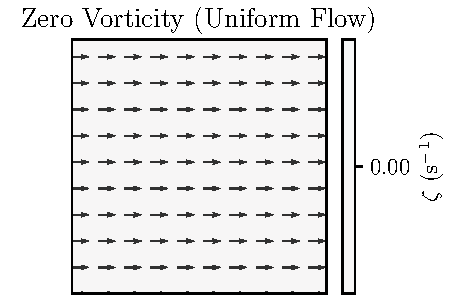
\includegraphics[]{papers/rossby/images/vorticity_plot0.pdf}

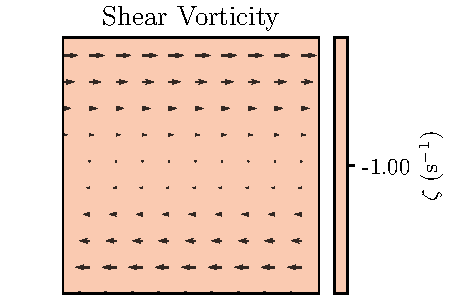
\includegraphics[]{papers/rossby/images/vorticity_plot1.pdf}

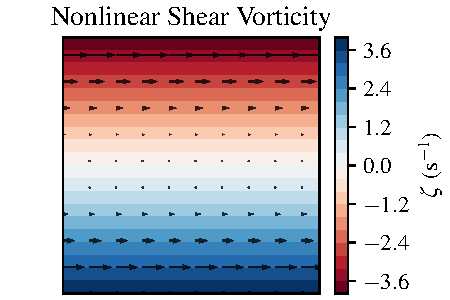
\includegraphics[]{papers/rossby/images/vorticity_plot2.pdf}

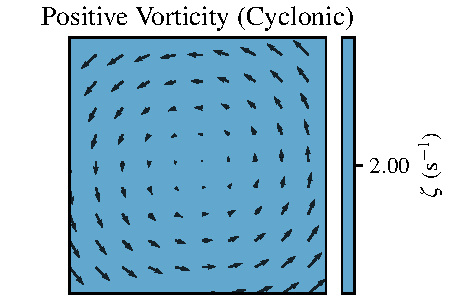
\includegraphics[]{papers/rossby/images/vorticity_plot3.pdf}

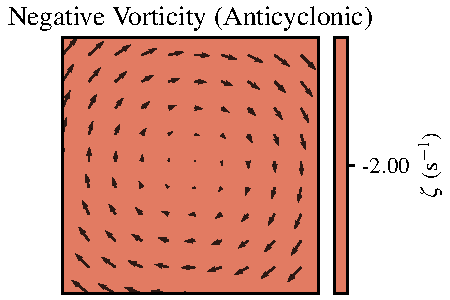
\includegraphics[]{papers/rossby/images/vorticity_plot4.pdf}


\tdplotsetmaincoords{70}{120}
\usepackage{tikz-3dplot}
\begin{tikzpicture}[tdplot_main_coords, scale=2]

  % Draw sphere
  \shade[ball color=blue!20, opacity=0.7] (0,0,0) circle (1);
  
  % Axes
  \draw[->] (0,0,0) -- (1.4,0,0) node[anchor=north east]{$x$};
  \draw[->] (0,0,0) -- (0,1.4,0) node[anchor=north west]{$y$};
  \draw[->] (0,0,0) -- (0,0,1.4) node[anchor=south]{$z$};
  
  % Latitude and Longitude (equator and meridian)
  \draw[dashed] (0,0,0) circle (1); % equator
  \tdplotdrawarc[tdplot_rotated_coords]{(0,0,0)}{1}{0}{180}{}{} % prime meridian
  
  % Tangent plane
  \filldraw[gray!40, opacity=0.7] (-0.4,-0.3,1) -- (0.4,-0.3,1) -- (0.4,0.3,1) -- (-0.4,0.3,1) -- cycle;
  \draw[->, thick] (0,0,1) -- (0,0,1.4) node[anchor=south]{$\vec{\Omega}$};
  \draw[->, thick] (0,0,1) -- (0.3,0.3,1) node[anchor=west]{$\beta$};
  
  % Label
  \node at (0.6,0.6,1.05) {tangent $\beta$-plane};
  
  \end{tikzpicture}

\printbibliography[heading=subbibliography]
\end{refsection}
